
\documentclass[12pt,a4paper]{article}

\usepackage{pdflscape}
\setlength{\textwidth}{165mm}
\setlength{\textheight}{235mm}
\setlength{\oddsidemargin}{-0mm}
\setlength{\topmargin}{-10mm}
\usepackage{caption}
\usepackage{mathtools}
\DeclarePairedDelimiter\abs{\lvert}{\rvert}%
\DeclarePairedDelimiter\norm{\lVert}{\rVert}%
% Swap the definition of \abs* and \norm*, so that \abs
% and \norm resizes the size of the brackets, and the
% starred version does not.
\makeatletter
\let\oldabs\abs
\def\abs{\@ifstar{\oldabs}{\oldabs*}}
%
\let\oldnorm\norm
\def\norm{\@ifstar{\oldnorm}{\oldnorm*}}
\makeatother

\newcommand*{\Value}{\frac{1}{2}x^2}%
%\usepackage{graphicx}
\usepackage{graphicx}
\usepackage{subfigure}%exclusive to subcaption
%\usepackage{subcaption, float} 
\usepackage{xcolor}
\definecolor{ggray}{RGB}{47,79,79}
\definecolor{firebrick}{RGB}{178,34,34}
\definecolor{green1}{RGB}{50,205,50}
\definecolor{umbrella}{RGB}{0,191,255}

\usepackage{pgfplots}
\usepackage{tikz}
\usetikzlibrary{patterns,arrows,shapes,positioning,shadows,trees}
\tikzstyle{every node}=[draw=black,thick,anchor=west]
\tikzstyle{selected}=[draw=red,fill=red!30]
\tikzstyle{optional}=[dashed,fill=gray!50]
\tikzstyle{neglected}=[dashed]

\usepackage{amsfonts}
\usepackage{amssymb,amsmath} %  $\displaystyle \sum$ will print a bigger one Σ , like in equations  in amsmath package

\DeclareMathOperator{\sgn}{sgn}

\usepackage{soul}

\usepackage{titlesec}
\titleformat*{\section}{\Large\sffamily}
\titleformat*{\subsection}{\large\sffamily}
\titleformat*{\subsubsection}{\itshape \sffamily}


%\renewcommand{\refname}{參考文獻}
\usepackage[nottoc]{tocbibind}
%\settocbibname{參考文獻}
\usepackage{float}
\usepackage{multirow}
\usepackage{booktabs}
%\usepackage[square]{natbib}

\title{Numerical Analysis HW12: Non-linear Resistor Network}
\author{Ming-Chang Chiu 100060007}
\date{June 2, 2015}
\begin{document}
\maketitle
\fontsize{12}{20pt}\selectfont %本行指令第一個12是字體大小、第二個20是行距,selectfont一定要加才會發生效果。但此指令只對正文有效,註解無效

\section{Objective}
In this assignment, we are required to solve a resistor network like the following picture with each resistance non-linear. 
\begin{figure}[h!]
  \centering
     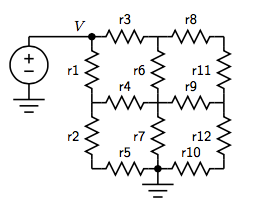
\includegraphics[width=0.4\textwidth]{./network.png}
  \caption{Resistor Network}
\end{figure}


I implementes genJ1(), genJ2(), genF1(), genF2() to generate the Jacobian matrix J and the system functions F. 
For Question 1, the resistance is voltage dependent, like:
\begin{figure}[h!]
  \centering
     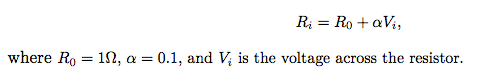
\includegraphics[width=0.6\textwidth]{./vq1.png}
\end{figure}

For Question 2, the resistance is temperature dependent, like:
\begin{figure}[h!]
  \centering
     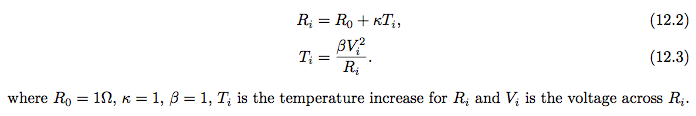
\includegraphics[width=0.8\textwidth]{./vq2.png}
\end{figure}
\section{Implementation}

The framework is basically as follow: 

\begin{figure}[h!]
  \centering
     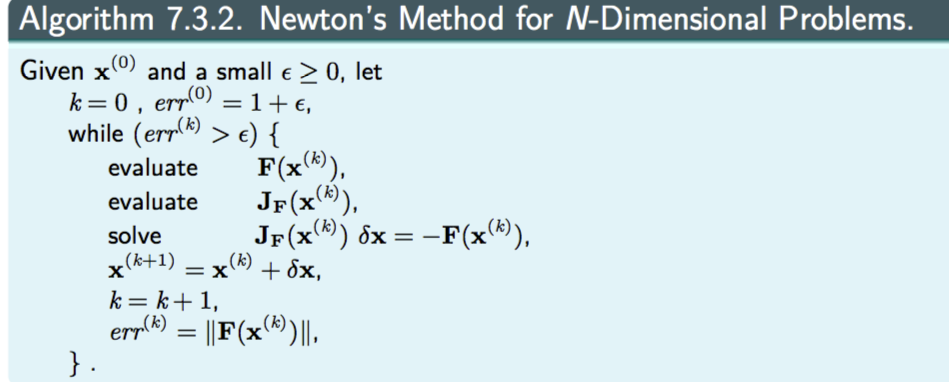
\includegraphics[width=0.8\textwidth]{./framework.png}
\end{figure}

and in function genJ1() and genJ2(), I just use the stamping method to create the Jacobian matrix. The tricky part in Q2 is to add entries for resistors to Jacobian matrix(i.e. in genJ2()).
To conquer this troublesome problem, I modify the order of resistors to the following graph:
\begin{figure}[h!]
  \centering
     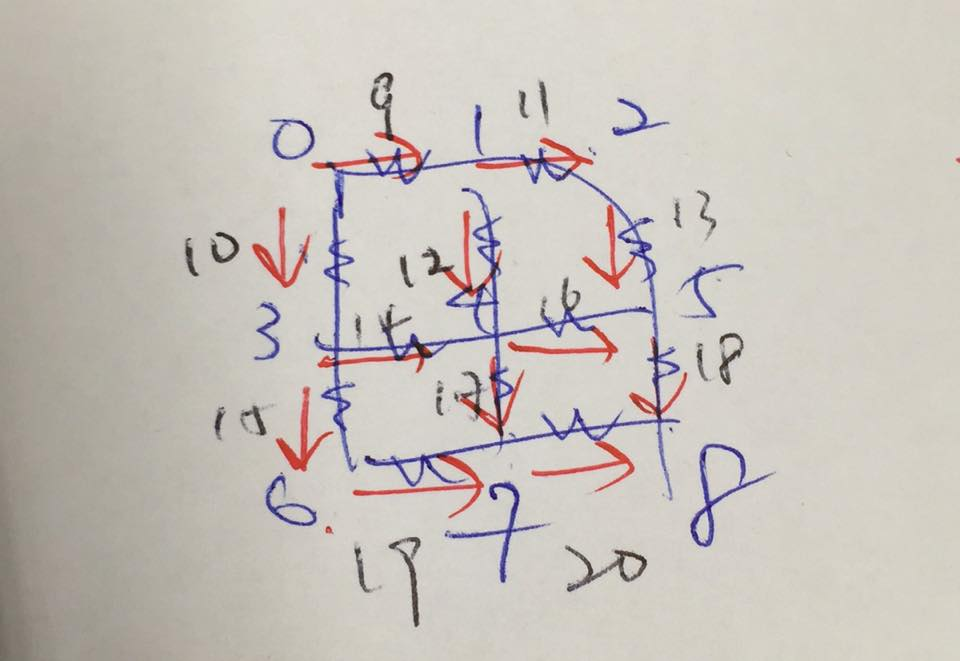
\includegraphics[width=0.4\textwidth]{./newnetwork.jpg}
\end{figure}
\\The blue numbers specify the node number and black numbers indicate the resistor numbers. The red arrows demonstrate the concept that how I do ordering on resistors. As for genF1() and genF2(),  they are meant to calculate the value of system functions, which are composed of Kichkoff's current equations or with the extension of temperature equation.Then, as we we have J and F, following the Newton's method, we can easily get the result.

And each entry my initial guesses are like [$v_0,v_1,v_2...,v_8,T_1,T_2....T_{12}$] for Q2, and [$v_0,v_1,v_2...v_8$] for Q1.

As for accuracy, I apply infinite norm on the system function F and the program will iterate until the norm is less than $10^{-8}$. 
\section{Workflow}
\begin{description}  

\item [Usage:] ./hw12.out  $\delta$, where $\delta$ could be 1 or 2 in this assignment, specifying Question 1 or 2 . For example,  ./hw12.out  2 
\item [Solve:] Newton's method is applied
\item[Desired output:] The program shall create data1.txt for Q1 with the first column is the voltage, second column is the total current, third column is the current of resistor 2, fourth column is the current of resistor 7, fifth column is the current of resistor 12 in figure 1. The program shall also can generate data2.txt for Q2 with the first column is the voltage, second column is the total current, third column is the temperature increase of resistor 2, fourth column is the temperature increase of resistor 7, fifth column is the temperature increase of resistor 12 in figure 1.
\end{description}

\section{Result and Plots}

In this report, I attach the numerical result at appendix section. One can also easily get the numerical data by running my program if interested.

\begin{figure}[h!]
  \centering
     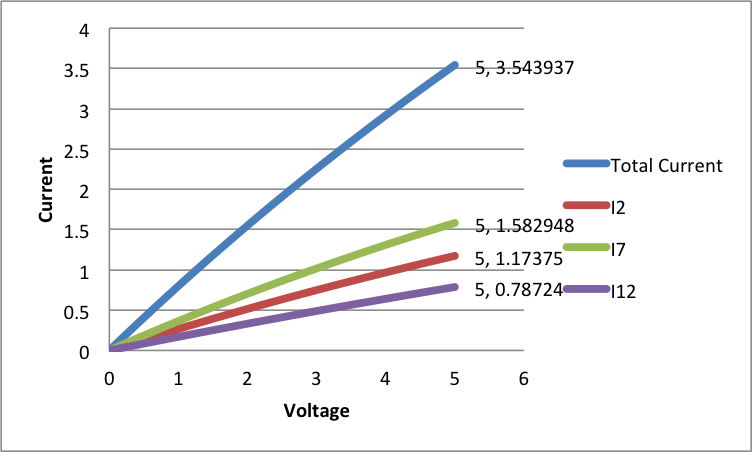
\includegraphics[width=0.9\textwidth]{./q1.png}
  \caption{Voltage-Current Plot for Q1}
\end{figure}
\newpage
\begin{figure}[h!]
  \centering
     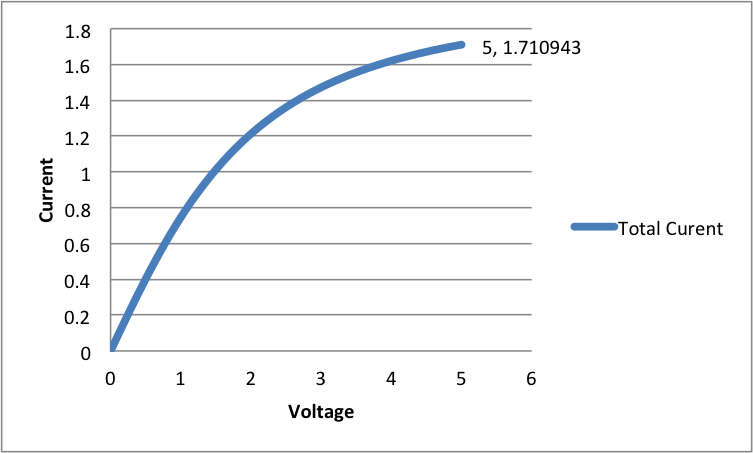
\includegraphics[width=0.9\textwidth]{./q21.png}
  \caption{Voltage-Current Plot for Q2}
\end{figure}
\begin{figure}[h!]
  \centering
     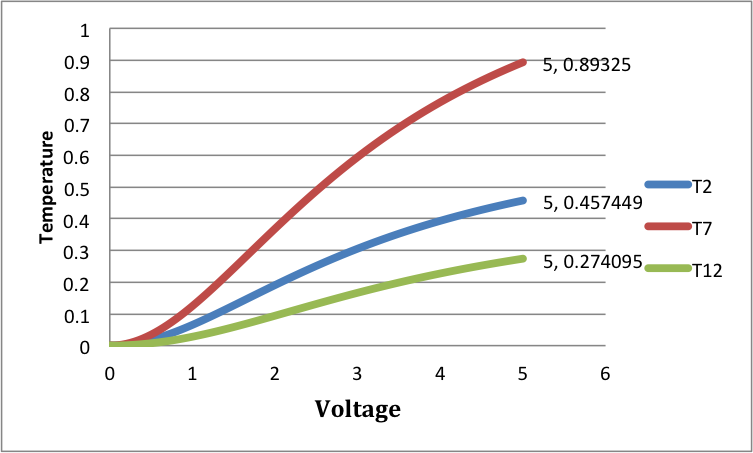
\includegraphics[width=0.9\textwidth]{./q22.png}
  \caption{Voltage-Temperature Increase Plot for Q2}
\end{figure}

\section{Observations}

When checking the correctness of this assignment, one can check if the total current equals  $I_2 + I_7 + I_{12}$. 

For Q1, the currents tend to increase linearly. $I_7$ is greater than $I_2$ and $I_2$ is greater than $I_{12}$.

For Q2, the total current will grow and the tend to saturate. Similarly, the temperature increase of resistor 7 in fig.1 is greater than resistor 2, resistor 2 is greater than resistor 12. 
\newpage
\section{Appendix}

\begin{figure}[h!]
  \centering
     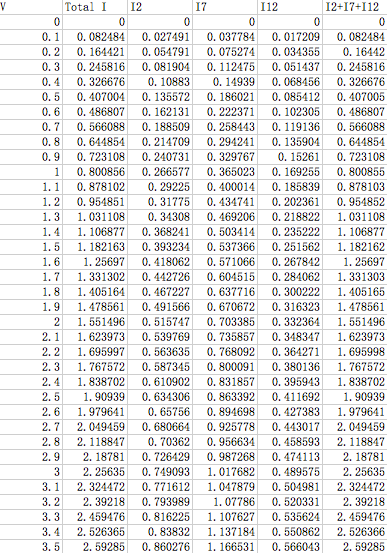
\includegraphics[width=0.7\textwidth]{./q11numerical.png}
  \caption{Q1 numerical data}
\end{figure}
\begin{figure}[h!]
  \centering
     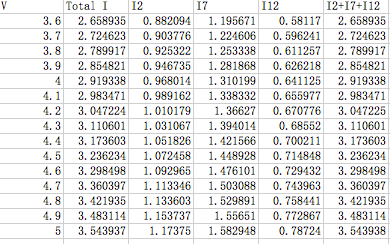
\includegraphics[width=0.7\textwidth]{./q12numerical.png}
  \caption{Q1 numerical data(continued)}
\end{figure}
\begin{figure}[h!]
  \centering
     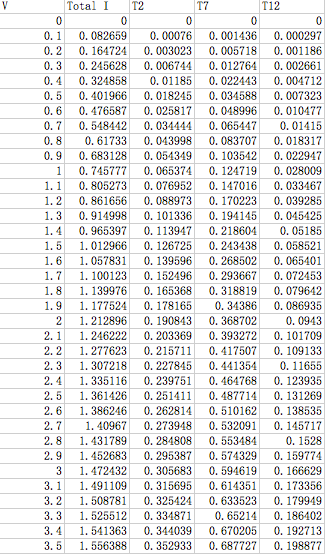
\includegraphics[width=0.65\textwidth]{./q21numerical.png}
  \caption{Q2 numerical data}
\end{figure}
\begin{figure}[h!]
  \centering
     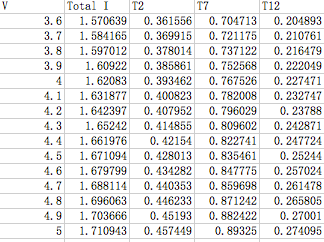
\includegraphics[width=0.65\textwidth]{./q22numerical.png}
  \caption{Q2 numerical data(continued)}
\end{figure}

\end{document} 
